\chapter{Introdução}
Num mundo altamente mecanizado, a força e o torque dentro de todas as grandezas, são as mais comuns. Estas têm um papel significativo nos aparelhos de medição de massa e células de carga usadas na indústria e retalho, nos automóveis e nas aeronaves, no aperto de tampas de frascos de medicina e parafusos.\cite{book-9}
\\
\\
A massa é uma das grandezas fundamentais, uma propriedade intrínseca de um objeto, que se mede pela sua resistência à aceleração.\cite{book-2}
%melhorar imagen
\begin{figure}[H]
	\centering
	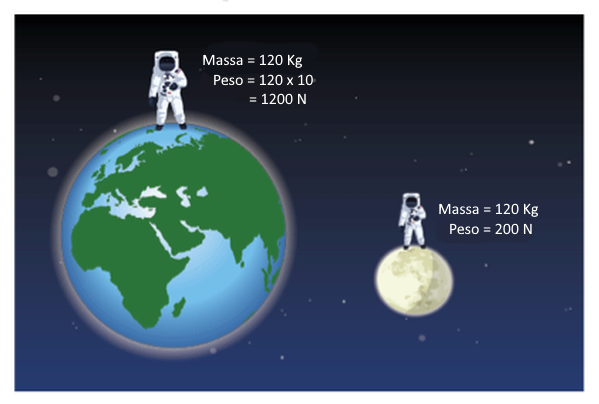
\includegraphics[width=.8\linewidth]{./image/PESTA/fisica/mass-1.png}
	\caption{Peso e Massa}
	\label{mass}
\end{figure}
Através da medição do peso, isto é, da força gravitacional exercida num dado objeto, podemos calcular a massa. \cite{book-2}
\\
\\
A massa dos objetos pode ser medida por balanças utilizando vários métodos, tais como as alavancas convencionais, por  molas e sistemas mais modernos, tais como, balanças digitais.
\\
\\
As balanças digitais estão presentes no nosso dia a dia, e tornaram-se numa ferramenta indispensável na indústria, comércio e laboratórios. Determinar a massa dos objetos facilitou a moeda de troca no comércio, e tornou-se num pilar fundamental da física e seu desenvolvimentos. Existe uma demanda, tanto na área comercial como na industrial, que empurra o desenvolvimento dos sensores para obter melhores resultados quanto a precisão e imunidade de influências exteriores na medição das grandezas mencionadas.
\\
\\
A importância desta grandeza (massa), foi o mote para o projeto proposto: a implementação de uma balança digital para uso doméstico, usando os meios que estão disponíveis no mercado.
%%%%%%%%%%%%%%%%%%%%%%%%%%%%%%%%%%%%%%%%%%%%%%%%%%%%%%%%%%
\section{Objetivos}
O objetivo principal deste projeto será a implementação de uma balança digital economicamente viável, usando os sensores e equipamentos disponíveis no mercado, para ter um produto útil e fácil de ser replicado.
\\
\\
Escolher o sensor adequado e meios de tratamento da informação e comunicação, será o objeto de estudo. Tendo como foco a utilização de um \textit{Embeded System} utilizando as ferramentas necessárias para o executar.
\\
\\
No final do produto obtido será testado, de forma a tentar aperfeiçoar, fazer melhorias, alterações e adaptações que possam surgir, de forma a simplificar o projeto e torná-lo mais atraente ao consumidor.
%%%%%%%%%%%%%%%%%%%%%%%%%%%%%%%%%%%%%%%%%%%%%%%%%%%%%%%%%%
\section{Calendarização}
O segundo semestre teve inicio em 8 de Março, num ambiente de pandemia COVID-19 período durante o qual fomos forçados ao ensino à distancia, e todo o trabalho teve de ser acompanhado \textit{online} pelos docentes. No entanto foi necessário organizar as tarefas pretendidas de acordo com o plano abaixo descrito, para poder fazer a entrega deste trabalho antes da data limite da época normal (28 de Junho de 2021).
\begin{table}[H]
	\caption{Calendarização das tarefas}
	%\begin{sidewaysfigure}
	\begin{ganttchart}[vgrid, hgrid]{1}{20}
		\gantttitle{Março}{5} 
		\gantttitle{Abril}{5}
		\gantttitle{Maio}{5}
		\gantttitle{Juno}{5}\\
		\gantttitlelist{1,...,20}{1}\\
		%First Group
		\ganttgroup{Requisitos}{2}{10} \\
		\ganttbar{Material}{3}{5} \\
		\ganttbar{\textit{Template} LaTeX}{5}{10} \\
		\ganttbar{\textbf{IDE} \textit{Template}}{3}{10}\\
		%\ganttlink{elem0}{elem1}
		%\ganttlink{elem1}{elem2}
		%\ganttlink{elem2}{elem3}
		%\ganttmilestone{Milestone 1}{11}
		%Second Group
		\ganttgroup{Projecto}{3}{20} \\
		\ganttbar{Kit Desenvolvimento}{3}{4} \\
		\ganttbar{Montagen Mesa Sensor}{5}{7} \\%5 7
		\ganttbar{HX711 comunicação}{4}{10} \\%4 8
		\ganttbar{Programação e ensaio}{4}{20}\\
		%\ganttlink{elem4}{elem5}
		%\ganttlink{elem5}{elem6}
		%\ganttlink{elem6}{elem7}
		%\ganttmilestone{Milestone 1}{11}
		%Third Group
		\ganttgroup{Relatório}{9}{20} \\
		\ganttbar{Literatura}{8}{12} \\
		\ganttbar{Análise documentação}{9}{12} \\
		%\ganttbar{Validação}{10}{12} \\
		\ganttbar{Execução}{10}{20}
		%\ganttlink{elem8}{elem9}
		%\ganttlink{elem9}{elem10}
		%\ganttlink{elem10}{elem11}
		%\ganttmilestone{Milestone 1}{11}
	\end{ganttchart}
	\label{gantt}
%\end{sidewaysfigure}
\end{table}
%%%%%%%%%%%%%%%%%%%%%%%%%%%%%%%%%%%%%%%%%%%%%%%%%%%%%%%%%%
\section{Organização do Relatório}
No capítulo 1 é feita uma contextualização do trabalho realizado e do seu propósito face às necessidades do mundo atual.
\\
\\
No capítulo 2 é apresentada uma breve história da evolução das balanças, e depois um estudo da balança eletrónica.
\\
\\
No capitulo 3 é apresentado a balança digital, seus componentes e características com uma descrição.
\\
\\
No capitulo 4 é descrito o software utilizado, estrutura do programa, e a implementação do código.
\\
\\
O capitulo 5 é a validação da implementação do projeto e seu funcionamento.
\\
\\
O capitulo 6 são expostos as conclusões e futuras possíveis alterações de melhoramento do produto.
%%%%%%%%%%%%%%%%%%%%%%%%%%%%%%%%%%%%%%%%%%%%%%%%%%%%%%%%%%